\section{Diode in a series}

Tương tự như exercise 1, xác định giá trị của điện áp \(V_{D1}, V_{D2}, V_{D3}\) và dòng điện I cho mạch. Sau đó, mô phỏng mạch sử dụng PSpice. Tuy nhiên, trong trường hợp này, mô hình diode thực tế phân cực thuận được sử dụng với điện áp ngưỡng \(V_{F} = 0.7223V\) .

\subsection{Tính toán theo lý thuyết}   

Dựa vào công thức tính cho mô hình diode thực tế:
    
    Ta có: 
\begin{itemize}
    
    \item \(V_{D1} = 10 - V_{F} = 10 - 0.7223 = 9.2777V\)

    \item \(V_{D2} = 10 - 2V_{F} = 10 - 2 \times 0.7223 = 8.5554 V\)

    \item \(V_{D3} = 10 - 3V_{F} = 10 - 3 \times 0.7223 = 7.8331 V\)
    
    \item \(V_{R1} = 10 - 3V_{F} = 10 - 3 \times 0.7223 = 7.8331 V\)
    
\end{itemize}

Công thức tính dòng điện \(I\):
\[
    I = \frac{V_{R1}}{R} = \frac{7.8331}{1000} = 7.8331 mA
\]
\subsection{Mô phỏng PSpice}

\begin{figure}[!htbp]
    \centering
    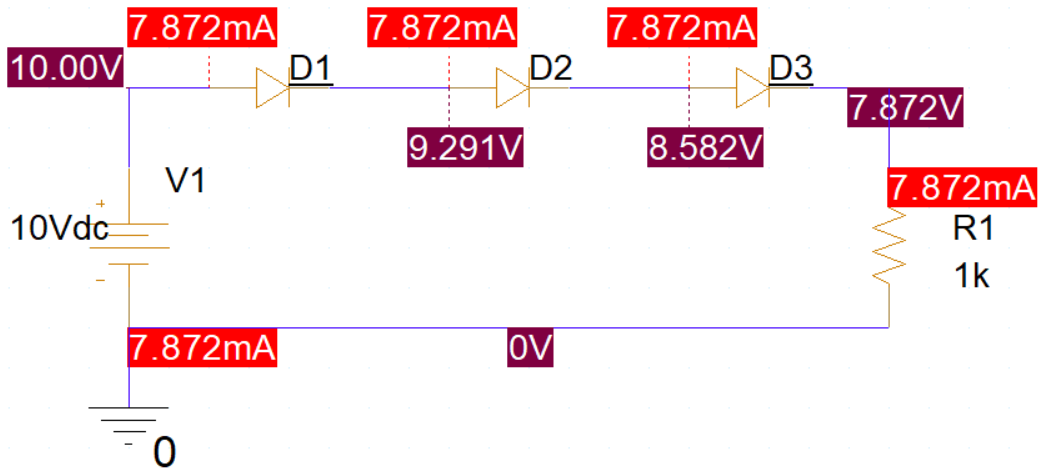
\includegraphics[width=0.8\textwidth]{graphics/ex2/f1.png}
    % \caption{Mạch mô phỏng trên PSpice}
\end{figure}

\subsubsection{So sánh}

% \FloatBarrier % Đảm bảo bảng không bị di chuyển lên trên

\begin{table}[H]
\centering

\begin{tabular}{|c|c|c|c|c|c|}
\hline
     & $V_{D1}$ & $V_{D2}$ & $V_{D3}$ & $V_{R1}$ & $I$  \\ \hline
Tính toán & 9.2777V &8.5554V &7.8331V &7.8331V &7.8331mA\\ \hline
PSpice      &9.291V &8.582V &7.872V &7.872V &7.872mA \\ \hline
\end{tabular}
\end{table}

Mạch trong bài tập này là một giải pháp đơn giản để thiết kế nguồn điện bằng cách tận dụng sự sụt áp của một diode. Ví dụ, một module SIM được sử dụng để gửi tin nhắn SMS có nguồn điện tốt ở mức 4.3V. Trong trường hợp này, một diode được kết nối từ nguồn 5V (một điện áp rất phổ biến) và sau đó, được kết nối với module SIM. Không chỉ được sử dụng để bảo vệ module tránh dòng ngược, diode còn là một giải pháp chi phí thấp để tạo ra nguồn điện 4.3V cho module SIM.